\documentclass[10pt]{article}
\usepackage[polish]{babel}
\usepackage[utf8]{inputenc}
\usepackage[T1]{fontenc}
\usepackage{amsmath}
\usepackage{amsfonts}
\usepackage{amssymb}
\usepackage[version=4]{mhchem}
\usepackage{stmaryrd}
\usepackage{graphicx}
\usepackage[export]{adjustbox}
\graphicspath{ {./images/} }

\title{EGZAMIN MATURALNY W ROKU SZKOLNYM 2016/2017 }

\author{ZASADY OCENIANIA ROZWIĄZAŃ ZADAŃ ARKUSZ MMA-R1}
\date{}


\begin{document}
\maketitle
FORMUŁA OD 2015\\
(,NOWA MATURA")

Uwaga: Akceptowane sq wszystkie odpowiedzi merytorycznie poprawne i spetniajace warunki zadania.

Zadanie 1. (0-1)

\begin{center}
\begin{tabular}{|l|l|c|}
\hline
\multicolumn{1}{|c|}{Wymagania ogólne} & \multicolumn{1}{c|}{Wymagania szczególowe} & \begin{tabular}{l}
Poprawna \\
odp. (1 p.) \\
\end{tabular} \\
\hline
\begin{tabular}{l}
II. Wykorzystanie \\
i interpretowanie \\
reprezentacji. \\
\end{tabular} & \begin{tabular}{l}
2. Wyrażenia algebraiczne. Zdajacy używa wzorów \\
skróconego mnożenia na $(a \pm b)^{2}$ oraz $a^{2}-b^{2}(2.1)$. \\
\end{tabular} & A \\
\hline
\end{tabular}
\end{center} \begin{tabular}{l}
1. Liczby rzeczywiste. Zdający posługuje się \\
w obliczeniach pierwiastkami dowolnego stopnia \\
i stosuje prawa działań na pierwiastkach (1.3). \\
\end{tabular}\$\textbackslash quad\textbackslash left\{\textbackslash begin\{array\}\{l\} \\


\textbackslash hline\textbackslash end\{array\}\textbackslash right.\$

Zadanie 2. (0-1)

\begin{center}
\begin{tabular}{|l|l|l|}
\hline
\begin{tabular}{l}
I. Wykorzystanie \\
i tworzenie informacji. \\
\end{tabular} & \begin{tabular}{l}
5. Ciągi. Zdający oblicza granice ciągów, korzystając \\
z granic ciągów typu $1 / n, 1 / n^{2}$ oraz z twierdzeń \\
o działaniach na granicach ciągów; (R5.2). \\
\end{tabular} & D \\
\hline
\end{tabular}
\end{center}

Zadanie 3. (0-1)

\begin{center}
\begin{tabular}{|l|l|l|}
\hline
\begin{tabular}{l}
IV. Użycie i tworzenie \\
strategii. \\
\end{tabular} & \begin{tabular}{l}
7. Planimetria. Zdający stosuje zależności między \\
kątem środkowym i kątem wpisanym; (7.1). \\
\end{tabular} & C \\
\hline
\end{tabular}
\end{center}

Zadanie 4. (0-1)

\begin{center}
\begin{tabular}{|l|l|l|}
\hline
\begin{tabular}{l}
II. Wykorzystanie \\
i interpretowanie \\
reprezentacji. \\
\end{tabular} & \begin{tabular}{l}
8. Geometria na płaszczyźnie kartezjańskiej. Zdający \\
oblicza współrzędne oraz długość wektora; dodaje \\
i odejmuje wektory oraz mnoży je przez liczbę. \\
\end{tabular} & B \\
\begin{tabular}{l}
Interpretuje geometrycznie działania na wektorach \\
(R8.7). \\
\end{tabular} & B &  \\
\hline
\end{tabular}
\end{center}

\section*{Zadanie 5. (0-2)}
\begin{center}
\begin{tabular}{|l|l|l|}
\hline
\begin{tabular}{l}
II. Wykorzystanie \\
i interpretowanie \\
reprezentacji. \\
\end{tabular} & \begin{tabular}{l}
3. Równania i nierówności. Zdający stosuje \\
twierdzenie o reszcie $z$ dzielenia \\
wielomianu przez dwumian $x-a($ R3.4 $)$. \\
\end{tabular} & $\mathbf{1 2 5}$ \\
\hline
\end{tabular}
\end{center}

Zadanie 6. (0-3)\\
II. Wykorzystanie i interpretowanie reprezentacji.\\
11. Rachunek różniczkowy. Zdający oblicza pochodne funkcji wymiernych oraz korzysta z geometrycznej i fizycznej interpretacji pochodnej (R11.2, R11.3).

\section*{Przykładowe rozwiązanie}
Pochodna funkcji $f$ jest równa

$$
f^{\prime}(x)=\frac{x^{2}+1-2 x(x-1)}{\left(x^{2}+1\right)^{2}}=\frac{-x^{2}+2 x+1}{\left(x^{2}+1\right)^{2}} \text { dla każdej liczby rzeczywistej } x
$$

Współczynnik kierunkowy szukanej stycznej jest równy:

$$
f^{\prime}(1)=\frac{2}{4}=\frac{1}{2},
$$

zatem równanie stycznej do wykresu funkcji $f \mathrm{w}$ punkcie $P=(1,0)$ ma postać:

$$
\begin{gathered}
y=\frac{1}{2}(x-1)+0 \\
y=\frac{1}{2} x-\frac{1}{2}
\end{gathered}
$$

\section*{Schemat punktowania}
\section*{Zdający otrzymuje}
1 p.\\
gdy wyznaczy pochodną funkcji $f$ :\\
np. $f^{\prime}(x)=\frac{x^{2}+1-2 x(x-1)}{\left(x^{2}+1\right)^{2}}$ lub $f^{\prime}(x)=\frac{-x^{2}+2 x+1}{\left(x^{2}+1\right)^{2}}$\\
i na tym zakończy lub dalej popełnia błędy.\\
Zdający otrzymuje\\
gdy obliczy $f^{\prime}(1)=\frac{1}{2}$, poprawnie interpretuje tę liczbę jako współczynnik kierunkowy stycznej i na tym zakończy lub dalej popełnia błędy.\\
Zdający otrzymuje 3 p.\\
gdy zapisze równanie stycznej do wykresu funkcji $f$ w punkcie $P=(1,0): \quad y=\frac{1}{2} x-\frac{1}{2}$.

\section*{Uwaga}
Jeżeli zdający wyznacza błędnie pochodną funkcji, np.: $\quad f^{\prime}(x)=\frac{x^{2}+1-2 x(x-1)}{x^{2}+1}$ i konsekwentnie do popełnionego błędu wyznaczy równanie stycznej, to otrzymuje $\mathbf{1}$ punkt.

\section*{Zadanie 7. (0-3)}
V. Rozumowanie i argumentacja.\\
2. Wyrażenia algebraiczne. Zdający używa wzorów skróconego mnożenia na $(a \pm b)^{2}$ oraz $a^{2}-b^{2}$ (2.1).\\
Zdający dodaje, odejmuje, mnoży i dzieli wyrażenia wymierne (R2.6).

\section*{Przykładowe rozwiązania}
\section*{I sposób}
Przekształcamy nierówność równoważnie:

$$
\begin{gathered}
x^{2} y^{2}-4 x y+4+2 x^{2}-4 x y+2 y^{2}>0 \\
(x y-2)^{2}+2\left(x^{2}-2 x y+y^{2}\right)>0 \\
(x y-2)^{2}+2(x-y)^{2}>0
\end{gathered}
$$

Ponieważ $x \neq y$, więc $(x-y)^{2}>0$. Zatem lewa strona tej nierówności jest sumą liczby nieujemnej $(x y-2)^{2}$ oraz liczby dodatniej $2(x-y)^{2}$, a więc jest dodatnia.\\
To kończy dowód.

\section*{II sposób}
Zapiszmy nierówność $x^{2} y^{2}+2 x^{2}+2 y^{2}-8 x y+4>0$ w postaci równoważnej

$$
\left(y^{2}+2\right) x^{2}-8 y \cdot x+2 y^{2}+4>0 .
$$

Ponieważ $y^{2}+2>0$ dla każdej liczby rzeczywistej $y$, więc możemy potraktować tę nierówność jak nierówność kwadratową z niewiadomą $x$ i parametrem $y$ (lub z niewiadomą $y$ i parametrem $x$ ). Wystarczy więc wykazać, że wyróżnik trójmianu kwadratowego $\left(y^{2}+2\right) x^{2}-8 y \cdot x+2 y^{2}+4$ zmiennej $x$ jest ujemny.

$$
\begin{aligned}
& \Delta=(-8 y)^{2}-4 \cdot\left(y^{2}+2\right) \cdot\left(2 y^{2}+4\right)=64 y^{2}-8\left(y^{2}+2\right)^{2}= \\
& =8\left(8 y^{2}-y^{4}-4 y^{2}-4\right)=8\left(-y^{4}+4 y^{2}-4\right)=-8\left(y^{2}-2\right)^{2} .
\end{aligned}
$$

Dla każdej liczby rzeczywistej $y$, takiej, że $y^{2} \neq 2$ wyróżnik jest ujemy. Gdy $y^{2}=2$, to wówczas nierówność $x^{2} y^{2}+2 x^{2}+2 y^{2}-8 x y+4>0$ ma postać

$$
\begin{aligned}
4 x^{2}-8 \sqrt{2} x+8 & >0 \text { lub } 4 x^{2}+8 \sqrt{2} x+8>0 \\
x^{2}-2 \sqrt{2} x+2 & >0 \text { lub } x^{2}+2 \sqrt{2} x+2>0 \\
(x-\sqrt{2})^{2} & >0 \text { lub }(x+\sqrt{2})^{2}>0
\end{aligned}
$$

Ponieważ z założenia wynika, że $x \neq y$, więc $x^{2} \neq 2$, a to oznacza, że każda z otrzymanych nierówności jest prawdziwa.\\
To kończy dowód.

\section*{III sposób}
Rozpatrzmy nierówność $x^{2} y^{2}+2 x^{2}+2 y^{2}-8 x y+4>0 \mathrm{w}$ trzech przypadkach.\\
I. Gdy co najmniej jedna z liczb $x, y$ jest równa 0 , np. gdy $x=0$. Wtedy nierówność przyjmuje postać

$$
2 y^{2}+4>0
$$

Ta nierówność jest prawdziwa dla każdej liczby rzeczywistej $y$.\\
II. Gdy żadna z liczb $x, y$ nie jest równa 0 i gdy $x y<0$. Wtedy po lewej stronie nierówności $x^{2} y^{2}+2 x^{2}+2 y^{2}-8 x y+4>0$ wszystkie składniki są dodatnie, więc nierówność jest prawdziwa.\\
III. Gdy żadna z liczb $x, y$ nie jest równa 0 i gdy $x y>0$. Wtedy, dzieląc obie strony nierówności $x^{2} y^{2}+2 x^{2}+2 y^{2}-8 x y+4>0$ przez $x y$, otrzymujemy nierówność równoważną

$$
\begin{gathered}
x y+2 \frac{x}{y}+2 \frac{y}{x}-8+\frac{4}{x y}>0 \\
x y+\frac{4}{x y}+2\left(\frac{x}{y}+\frac{y}{x}\right)-8>0 \\
x y-4+\frac{4}{x y}+2\left(\frac{x}{y}-2+\frac{y}{x}\right)>0 \\
\left(\sqrt{x y}-\frac{2}{\sqrt{x y}}\right)^{2}+2\left(\sqrt{\frac{x}{y}}-\sqrt{\frac{y}{x}}\right)^{2}>0
\end{gathered}
$$

Ponieważ z założenia $x \neq y$, więc $\frac{x}{y} \neq 1$, zatem $\frac{x}{y} \neq \frac{y}{x}$, co oznacza, że $\left(\sqrt{\frac{x}{y}}-\sqrt{\frac{y}{x}}\right)^{2}>0$.\\
Stąd i z tego, że $\left(\sqrt{x y}-\frac{2}{\sqrt{x y}}\right)^{2} \geq 0$ wynika prawdziwość otrzymanej nierówności.\\
To kończy dowód.

\section*{IV sposób}
I. Gdy $x y \leq 0$, to wtedy po lewej stronie nierówności $x^{2} y^{2}+2 x^{2}+2 y^{2}-8 x y+4>0$ cztery pierwsze składniki są nieujemne, piąty jest dodatni, więc nierówność jest prawdziwa.\\
II. Gdy $x y>0$, wtedy z nierówności między średnią arytmetyczną i geometryczną dla liczb dodatnich $x^{2} y^{2}, 2 x^{2}, 2 y^{2}$ i 4 otrzymujemy

$$
\frac{x^{2} y^{2}+2 x^{2}+2 y^{2}+4}{4} \geq \sqrt[4]{x^{2} y^{2} \cdot 2 x^{2} \cdot 2 y^{2} \cdot 4}=\sqrt[4]{16 x^{4} y^{4}}=2 x y
$$

skąd

$$
x^{2} y^{2}+2 x^{2}+2 y^{2}+4 \geq 8 x y .
$$

Równość miałaby miejsce tylko wtedy, gdyby $x^{2} y^{2}=2 x^{2}=2 y^{2}=4$, a więc gdyby $x^{2}=y^{2}$, co wobec nierówności $x y>0$ oznaczałoby $x=y$, co jest sprzeczne z założeniem. Zatem

$$
x^{2} y^{2}+2 x^{2}+2 y^{2}+4>8 x y
$$

czyli

$$
x^{2} y^{2}+2 x^{2}+2 y^{2}-8 x y+4>0
$$

To kończy dowód.

\section*{Schemat punktowania}
\section*{I sposób rozwiązania}
Pokonanie zasadniczych trudności zadania\\
Zdający zapisze nierówność w postaci $(x y-2)^{2}+2(x-y)^{2}>0$ i na tym zakończy lub dalej popełnia błędy.\\
Rozwiązanie pelne. 3 p.\\
Zdający przeprowadzi pełne rozumowanie, uwzględniające założenie, że $x \neq y$.\\
II sposób rozwiązania\\
Rozwiązanie, w którym postęp jest istotny\\
1 p.\\
Zdający zapisze nierówność w postaci $\left(y^{2}+2\right) x^{2}-8 y \cdot x+2 y^{2}+4>0$, obliczy wyróżnik trójmianu kwadratowego $\left(y^{2}+2\right) x^{2}-8 y \cdot x+2 y^{2}+4$, $\mathrm{np} .: \Delta=(-8 y)^{2}-4 \cdot\left(y^{2}+2\right) \cdot\left(2 y^{2}+4\right)$ i na tym zakończy lub dalej popełnia błędy.\\
Pokonanie zasadniczych trudności zadania\\
Zdający uzasadni, że wyróżnik $\Delta=-8\left(y^{2}-2\right)^{2}$ jest niedodatni dla każdej liczby rzeczywistej $y$, ale nie rozpatrzy przypadku, gdy $y^{2}=2$ i na tym zakończy lub dalej popełnia błędy.\\
Rozwiązanie pelne\\
3 p.\\
Zdający przeprowadzi pełne rozumowanie.\\
III sposób rozwiązania\\
Rozwiązanie, w którym postęp jest istotny\\
1 p.\\
Zdający wykaże prawdziwość nierówności w I i w II przypadku i na tym zakończy lub dalej popełnia błędy.\\
Pokonanie zasadniczych trudności zadania\\
2 p.\\
Zdający zapisze nierówność w postaci $x y+\frac{4}{x y}+2\left(\frac{x}{y}+\frac{y}{x}\right)-8>0$ w przypadku, gdy $x y>0$ i na tym zakończy lub dalej popełnia błędy.\\
Rozwiązanie pelne\\
Zdający przeprowadzi pełne rozumowanie.\\
IV sposób rozwiązania\\
Rozwiązanie, w którym postęp jest istotny 1 p.

Zdający wykaże prawdziwość nierówności $x^{2} y^{2}+2 x^{2}+2 y^{2}-8 x y+4>0$ w I przypadku i na tym zakończy lub dalej popełnia błędy.

Zdający uzasadni, że gdy $x y>0$, to prawdziwa jest nierówność $\frac{x^{2} y^{2}+2 x^{2}+2 y^{2}+4}{4} \geq 2 x y$ i na tym zakończy lub dalej popełnia błędy.\\
Rozwiązanie pełne 3 p.\\
Zdający przeprowadzi pełne rozumowanie.

Zadanie 8. (0-3)

\begin{center}
\begin{tabular}{|l|l|}
\hline
 & \begin{tabular}{l}
7. Planimetria. Zdający korzysta z własności funkcji \\
trygonometrycznych w łatwych obliczeniach geometrycznych, w tym \\
ze wzoru na pole trójkąta ostrokątnego o danych dwóch bokach \\
\end{tabular} \\
i kacie między nimi. (7.4). &  \\
V. Rozumowanie &  \\
i argumentacja. & \begin{tabular}{l}
Zdający rozpoznaje figury podobne i jednokładne wykorzystuje \\
(także w kontekstach praktycznych) ich własności. (R7.4). \\
Zdający znajduje związki miarowe w figurach płaskich \\
z zastosowaniem twierdzenia sinusów i twierdzenia cosinusów. \\
(R7.5). \\
\end{tabular} \\
\hline
\end{tabular}
\end{center}

\section*{Przykładowe rozwiązania}
I sposób\\
Przyjmijmy oznaczenia jak na rysunku.\\
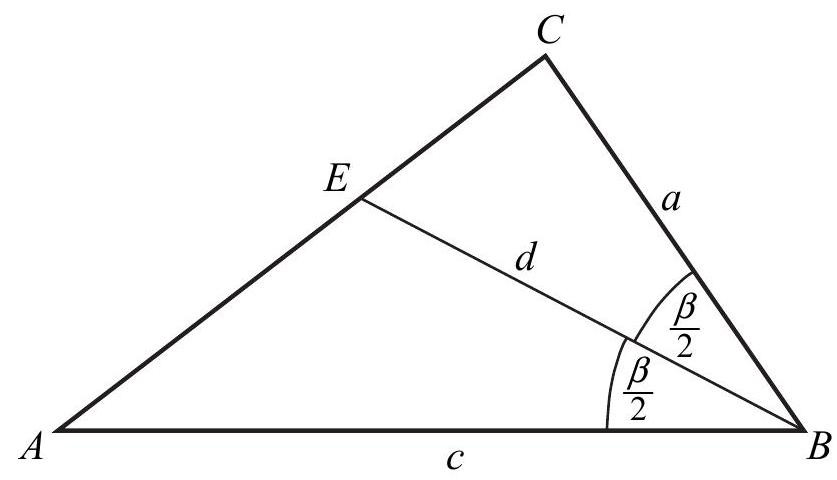
\includegraphics[max width=\textwidth, center]{2025_02_07_cd06b1485e4d114dda29g-07}

Pole trójkąta $A B C$ jest równe

$$
P_{A B C}=\frac{1}{2} a \cdot c \cdot \sin \beta .
$$

Pola trójkątów $A B E$ i $C B E$ są równe

$$
P_{A B E}=\frac{1}{2} d \cdot c \cdot \sin \frac{\beta}{2} \text { oraz } P_{C B E}=\frac{1}{2} d \cdot a \cdot \sin \frac{\beta}{2} .
$$

Suma pól trójkątów $A B E$ i $C B E$ jest równa polu trójkąta $A B C$, zatem

$$
\frac{1}{2} a \cdot c \cdot \sin \beta=\frac{1}{2} d \cdot c \cdot \sin \frac{\beta}{2}+\frac{1}{2} d \cdot a \cdot \sin \frac{\beta}{2} .
$$

Stąd

$$
\begin{gathered}
a \cdot c \cdot 2 \sin \frac{\beta}{2} \cos \frac{\beta}{2}=d \cdot(a+c) \cdot \sin \frac{\beta}{2} . \\
2 a c \cdot \cos \frac{\beta}{2}=d \cdot(a+c), \\
d=\frac{2 a c}{a+c} \cdot \cos \frac{\beta}{2} .
\end{gathered}
$$

To kończy dowód.\\
II sposób\\
Przyjmijmy oznaczenia jak na rysunku.\\
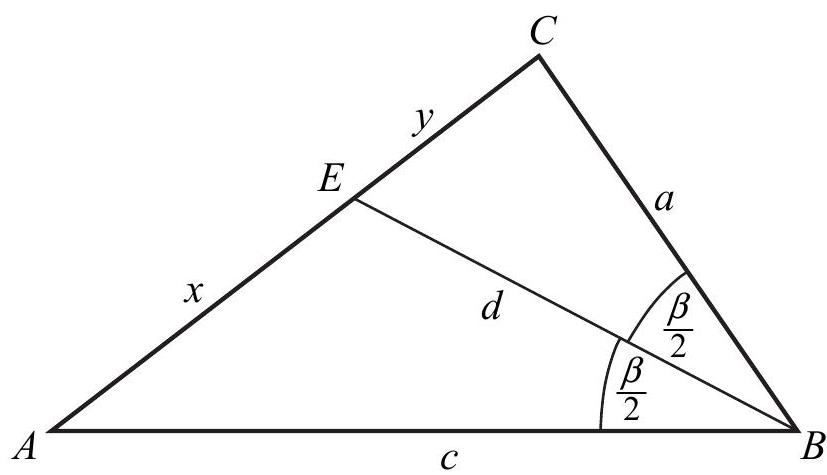
\includegraphics[max width=\textwidth, center]{2025_02_07_cd06b1485e4d114dda29g-08}

Z twierdzenia o dwusiecznej otrzymujemy

$$
\frac{|C E|}{|A E|}=\frac{|C B|}{|A B|}, \operatorname{czyli} \frac{y}{x}=\frac{a}{c} .
$$

Z twierdzenia cosinusów dla trójkątów $A B E$ i $C B E$ otrzymujemy

$$
x^{2}=c^{2}+d^{2}-2 c d \cos \frac{\beta}{2} \text { oraz } y^{2}=a^{2}+d^{2}-2 a d \cos \frac{\beta}{2} .
$$

Zatem

$$
\frac{a^{2}}{c^{2}}=\frac{y^{2}}{x^{2}}=\frac{a^{2}+d^{2}-2 a d \cos \frac{\beta}{2}}{c^{2}+d^{2}-2 c d \cos \frac{\beta}{2}} .
$$

Stąd otrzymujemy

$$
\begin{gathered}
a^{2}\left(c^{2}+d^{2}-2 c d \cos \frac{\beta}{2}\right)=c^{2}\left(a^{2}+d^{2}-2 a d \cos \frac{\beta}{2}\right), \\
a^{2} c^{2}+a^{2} d^{2}-2 a^{2} c d \cos \frac{\beta}{2}=a^{2} c^{2}+c^{2} d^{2}-2 a c^{2} d \cos \frac{\beta}{2}, \\
a^{2} d^{2}-c^{2} d^{2}=2 a^{2} c d \cos \frac{\beta}{2}-2 a c^{2} d \cos \frac{\beta}{2}, \\
\left(a^{2}-c^{2}\right) d=2(a-c) a c \cos \frac{\beta}{2} .
\end{gathered}
$$

Gdy $a=c$, wówczas trójkąt $A B C$ jest równoramienny, więc trójkąty $A B E$ i $C B E$ są\\
prostokątne i przystające. Wtedy $\cos \frac{\beta}{2}=\frac{d}{c}$, skąd $d=c \cos \frac{\beta}{2}=\frac{2 c^{2}}{2 c} \cos \frac{\beta}{2}=\frac{2 a c}{a+c} \cos \frac{\beta}{2}$.\\
Gdy zaś $a \neq c$, to $(a-c)(a+c) \neq 0$, czyli $a^{2}-c^{2} \neq 0$, więc

$$
d=\frac{2(a-c)}{a^{2}-c^{2}} a c \cos \frac{\beta}{2}=\frac{2 a c}{a+c} \cos \frac{\beta}{2} .
$$

To kończy dowód.

\section*{III sposób}
Poprowadźmy wysokości $C G$ i $E F$ trójkątów $A B C$ i $A B E$. Ponieważ trójkąt $A B C$ jest ostrokątny, więc spodki $F$ i $G$ tych wysokości leżą na boku $A B$ trójkąta $A B C$. Pozostałe oznaczenia przyjmijmy jak na rysunku.\\
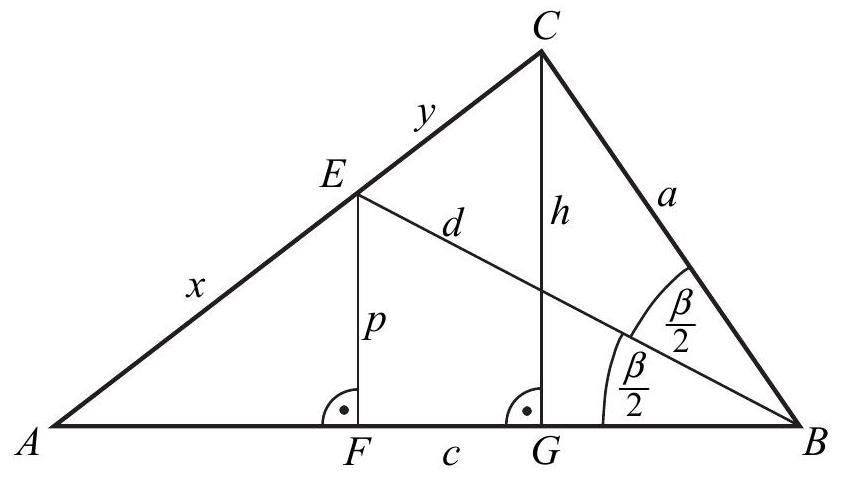
\includegraphics[max width=\textwidth, center]{2025_02_07_cd06b1485e4d114dda29g-09}

Z twierdzenia o dwusiecznej otrzymujemy

$$
\frac{|C E|}{|A E|}=\frac{|C B|}{|A B|} \text {, czyli } \frac{y}{x}=\frac{a}{c} .
$$

Z trójkątów $B E F$ i $B C G$ otrzymujemy

$$
\frac{p}{d}=\sin \frac{\beta}{2} \text { oraz } \frac{h}{a}=\sin \beta .
$$

Stąd

$$
p=d \sin \frac{\beta}{2} \text { oraz } h=a \sin \beta .
$$

Trójkąty $A F E$ i $A G C$ są podobne, gdyż oba są prostokątne i mają wspólny kąt ostry przy wierzchołku $A$. Zatem

$$
\frac{|E F|}{|A E|}=\frac{|C G|}{|A C|}, \operatorname{czyli} \frac{p}{x}=\frac{h}{x+y} .
$$

Stąd i z poprzednio otrzymanych równości otrzymujemy kolejno

$$
\begin{gathered}
\frac{d \sin \frac{\beta}{2}}{x}=\frac{a \sin \beta}{x+y}, \\
d \sin \frac{\beta}{2}=\frac{a \cdot 2 \sin \frac{\beta}{2} \cos \frac{\beta}{2}}{1+\frac{y}{x}}, \\
d=\frac{2 a \cdot \cos \frac{\beta}{2}}{1+\frac{a}{c}}=\frac{2 a c \cdot \cos \frac{\beta}{2}}{a+c} .
\end{gathered}
$$

To kończy dowód.

\section*{Schemat punktowania}
\section*{I sposób rozwiązania}
Rozwiązanie, w którym postęp jest istotny\\
1 p.\\
Zdający

\begin{itemize}
  \item zapisze pola każdego z trójkątów $A B C, A B E$ i $C B E$ w zależności od długości $a, c, d$ i kąta $\beta: P_{A B C}=\frac{1}{2} a \cdot c \cdot \sin \beta, P_{A B E}=\frac{1}{2} d \cdot c \cdot \sin \frac{\beta}{2}, P_{C B E}=\frac{1}{2} d \cdot a \cdot \sin \frac{\beta}{2}$\\
albo
  \item zapisze, że pole trójkąta $A B C$ jest sumą pól trójkątów $A B E$ i $C B E$ oraz zapisze jedno z tych pól: $P_{A B C}=\frac{1}{2} a \cdot c \cdot \sin \beta$ lub $P_{A B E}=\frac{1}{2} d \cdot c \cdot \sin \frac{\beta}{2}$ lub $P_{C B E}=\frac{1}{2} d \cdot a \cdot \sin \frac{\beta}{2}$\\
i na tym zakończy lub dalej popełnia błędy.\\
Pokonanie zasadniczych trudności zadania\\
2 p.\\
Zdający zapisze zależność między polem trójkąta $A B C$ i polami trójkątów $A B E$ i $C B E$ w postaci, w której występują jedynie wielkości $a, c, d$ i $\beta$, np.:
\end{itemize}

$$
\frac{1}{2} a \cdot c \cdot \sin \beta=\frac{1}{2} d \cdot c \cdot \sin \frac{\beta}{2}+\frac{1}{2} d \cdot a \cdot \sin \frac{\beta}{2}
$$

i na tym zakończy lub dalej popełnia błędy.

\section*{Rozwiązanie pełne}
Zdający przeprowadzi pełne rozumowanie.

\section*{II sposób rozwiązania}
Rozwiązanie, w którym postęp jest istotny\\
Zdający zapisze zależności między wielkościami $x, y, d, a$ i $c$ oraz kątem $\beta$ :

$$
\frac{y}{x}=\frac{a}{c}, x^{2}=c^{2}+d^{2}-2 c d \cos \frac{\beta}{2}, y^{2}=a^{2}+d^{2}-2 a d \cos \frac{\beta}{2}
$$

i na tym zakończy lub dalej popełnia błędy.\\
Pokonanie zasadniczych trudności zadania\\
Zdający zapisze równanie, np.: $\frac{a^{2}}{c^{2}}=\frac{a^{2}+d^{2}-2 a d \cos \frac{\beta}{2}}{c^{2}+d^{2}-2 c d \cos \frac{\beta}{2}}$\\
i na tym zakończy lub dalej popełnia błędy.

Rozwiązanie pelne\\
Zdający przeprowadzi pełne rozumowanie.

\section*{Uwaga}
Jeżeli zdający nie rozważy sytuacji gdy $a=c$, to może otrzymać co najwyżej $\mathbf{2}$ punkty.

\section*{III sposób rozwiązania}
\section*{Rozwiązanie, w którym postęp jest istotny}
\section*{Zdający zapisze}
\begin{itemize}
  \item zależność między wielkościami $x, y, a$ i $c$ oraz zależności między wielkościami $p, h \mathrm{i} a$ oraz kątem $\beta: \frac{y}{x}=\frac{a}{c}, \frac{p}{d}=\sin \frac{\beta}{2}, \frac{h}{a}=\sin \beta$\\
albo
  \item zależność między wielkościami $x, y, a$ i $c$ oraz zależności między wielkościami $p, h, x$ i $y$ oraz kątem $\beta: \frac{y}{x}=\frac{a}{c}, \frac{p}{x}=\frac{h}{x+y}$,\\
albo
  \item zależność między wielkościami $p, h$ i $a$ oraz kątem $\beta$ oraz zależność między wielkościami $x, y, a$ i $c: \frac{p}{d}=\sin \frac{\beta}{2}, \frac{h}{a}=\sin \beta, \frac{y}{x}=\frac{a}{c}$\\
i na tym zakończy lub dalej popełnia błędy.\\
Pokonanie zasadniczych trudności zadania\\
Zdający zapisze wystarczającą liczbę zależności między wielkościami $x, y, a, c, p$ i $h$ oraz kątem $\beta$, pozwalającą wyznaczyć $d$ w zależności od wielkości $a, c$ i kąta $\beta$, np.:
\end{itemize}

$$
\frac{y}{x}=\frac{a}{c}, \frac{d \sin \frac{\beta}{2}}{x}=\frac{a \sin \beta}{x+y}
$$

i na tym zakończy lub dalej popełnia błędy.\\
Rozwiązanie pełne 3 p.\\
Zdający przeprowadzi pełne rozumowanie.

\section*{Uwaga}
Jeżeli zdający zapisze jedynie 3 razy twierdzenie cosinusów, to otrzymuje $\mathbf{0}$ punktów.

\section*{Zadanie 9. (0-4)}
\begin{center}
\begin{tabular}{|l|l|}
\hline
 & \begin{tabular}{l}
9. Stereometria. Zdający określa, jaką figurą jest dany przekrój \\
graniastosłupa lub ostrosłupa płaszczyzną. (R9.2). \\
\end{tabular} \\
IV. Użycie i tworzenie &  \\
strategii. & \begin{tabular}{l}
7. Planimetria. Zdający rozpoznaje figury podobne i jednokładne; \\
wykorzystuje (także w kontekstach praktycznych) ich własności \\
(R7.4). \\
G10. Figury płaskie. Zdający stosuje twierdzenie Pitagorasa (G10.7). \\
\hline
\end{tabular} \\
\hline
\end{tabular}
\end{center}

\section*{Przykładowe rozwiązanie}
Niech $K$ będzie środkiem odcinka $B C$, a $M$ i $O$ spodkami wysokości trójkąta $A K D$ opuszczonymi z wierzchołków $A$ i $D$. Płaszczyzny $A K D$ i $A B C$ są prostopadłe, bo prosta $B C$ jest prostopadła do płaszczyzny $A K D$.\\
Niech $T$ będzie punktem wspólnym wysokości $A M$ i $D O$. Odległości punktu $T$ od prostych $A K$ i $D K$ są równe, bo $|A K|=|D K|$. Są to też odległości punktu $T$ od płaszczyzn $A B C$ i $B C D$. Ten sam punkt $T$ otrzymamy rozpatrując trójkąt $L C D$, gdzie $L$ jest środkiem odcinka $A B$ lub\\
trójkąt $\pounds B D$, gdzie $Ł$ jest środkiem odcinka $A C$. Wynika stąd, że odległość punktu $T$ od każdej ściany czworościanu $A B C D$ jest taka sama. Wobec tego $S=T$.

Niech $H$ oznacza wysokość czworościanu, $h$ wysokość ściany czworościanu, a $R$ - promień kuli, o której mowa w treści zadania. Pozostałe oznaczenia przyjmijmy takie jak na rysunku.\\
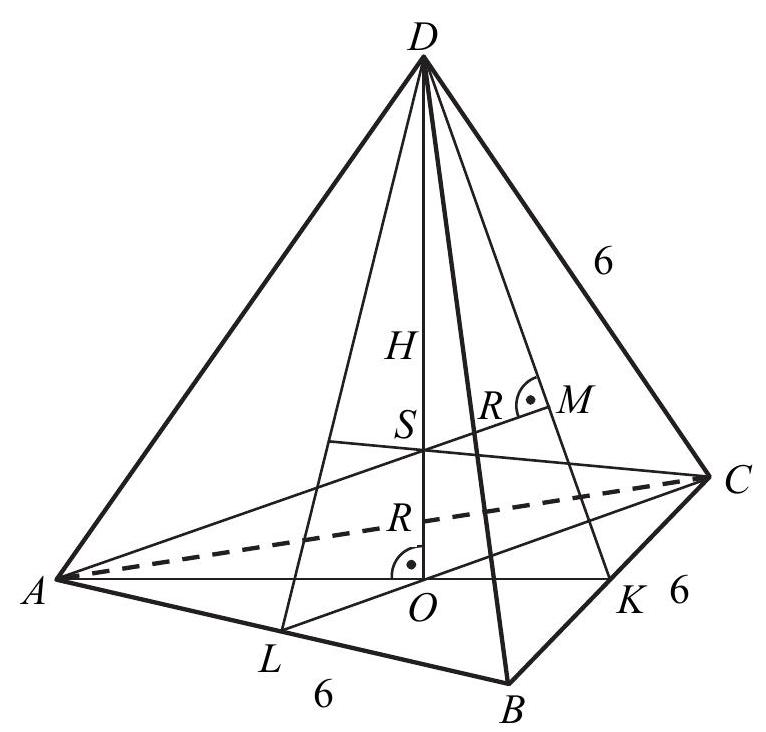
\includegraphics[max width=\textwidth, center]{2025_02_07_cd06b1485e4d114dda29g-12}

Wyznaczymy wysokość $H$ czworościanu.\\
Odcinki $A K$ i $D K$ to wysokości przystających trójkątów równobocznych $A B C$ i $B C D$ o boku długości 6 , więc

$$
|A K|=|D K|=\frac{6 \sqrt{3}}{2}=3 \sqrt{3} .
$$

Spodek $O$ wysokości $D O$ czworościanu jest środkiem ciężkości trójkąta $A B C$, więc

$$
|K O|=\frac{1}{3}|A K|=\sqrt{3}
$$

Z twierdzenia Pitagorasa dla trójkąta $D O K$ otrzymujemy

$$
\begin{aligned}
& |D O|^{2}+|K O|^{2}=|D K|^{2} \\
& H^{2}+(\sqrt{3})^{2}=(3 \sqrt{3})^{2} .
\end{aligned}
$$

Stąd

$$
\begin{gathered}
H^{2}=(3 \sqrt{3})^{2}-(\sqrt{3})^{2}, \\
H=2 \sqrt{6} .
\end{gathered}
$$

Wyznaczamy odległość $d$ środka $S$ kuli od płaszczyzny $\pi$.

\section*{I sposób}
Niech $P$ będzie punktem, w którym wysokość $D O$ przebija płaszczyznę $\pi$. Ponieważ płaszczyzna $\pi$ jest równoległa do płaszczyzny ściany $A B C$, więc czworościan odcięty tą płaszczyzną od czworościanu $A B C D$ jest podobny do czworościanu $A B C D$, a skala tego podobieństwa jest równa $\sqrt[3]{\frac{8}{27}}=\frac{2}{3}$. Wynika stąd, że płaszczyzna $\pi$ przecina wysokość $D K$ ściany bocznej $B C D$ w takim punkcie $M^{\prime}$, że

$$
\left|D M^{\prime}\right|=\frac{2}{3}|D K| .
$$

To oznacza $M^{\prime}=M$.\\
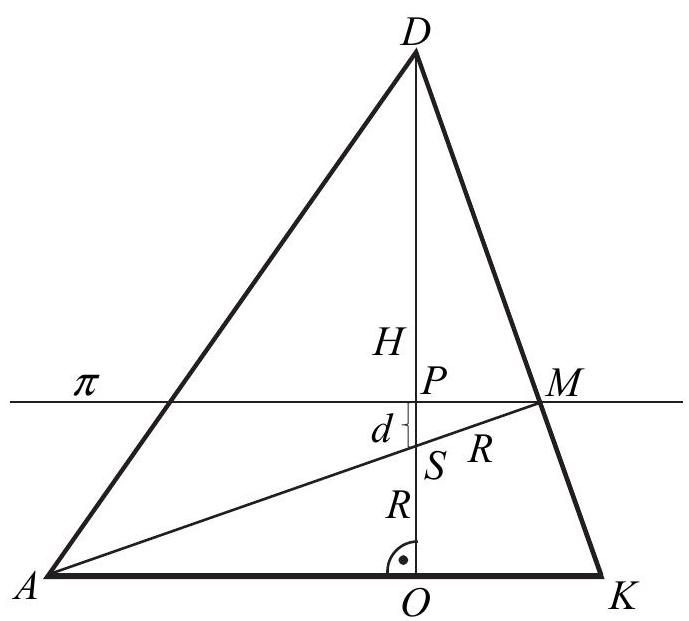
\includegraphics[max width=\textwidth, center]{2025_02_07_cd06b1485e4d114dda29g-13}

Trójkąty $D O K, D P M, M P S$ są podobne, ponieważ para trójkątów prostokątnych $D O K, D P M$ ma jeden kąt ostry wspólny oraz para trójkątów prostokątnych $D P M, M P S$ ma jeden kąt ostry wspólny. Zatem\\
Stąd

$$
\frac{|D P|}{|M P|}=\frac{|D O|}{|O K|}=\frac{|M P|}{|P S|}, \operatorname{czyli} \frac{\frac{2}{3} H}{|M P|}=\frac{H}{\sqrt{3}}=\frac{|M P|}{d} .
$$

Stąd

$$
|M P|=\frac{2}{3} \sqrt{3} \operatorname{oraz} \frac{2 \sqrt{6}}{\sqrt{3}}=\frac{\frac{2}{3} \sqrt{3}}{d}
$$

Zatem $d=\frac{\sqrt{6}}{6}$.

\section*{II sposób}
Obliczymy najpierw promień $R$ kuli.\\
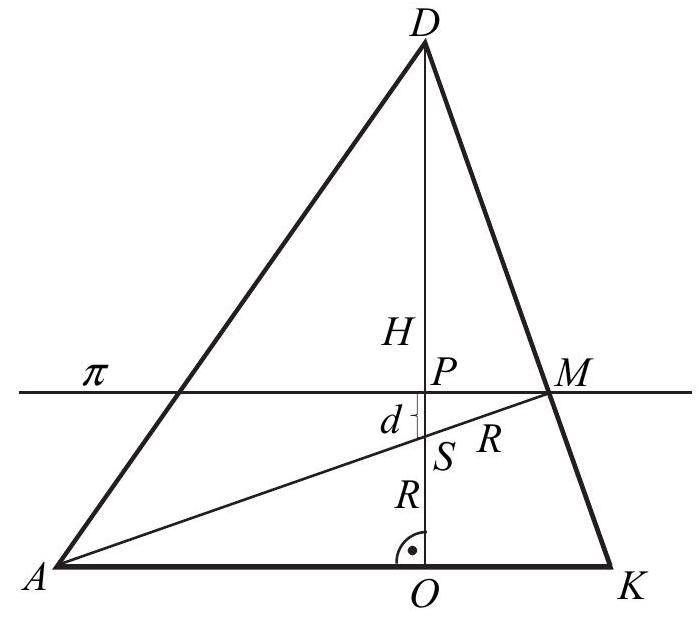
\includegraphics[max width=\textwidth, center]{2025_02_07_cd06b1485e4d114dda29g-14}

Trójkąty $D O K$ i $D M S$ są podobne, ponieważ są prostokątne i mają jeden kąt ostry wspólny.\\
Zatem $\frac{|S M|}{|D S|}=\frac{|K O|}{|D K|}$. Stąd

$$
\begin{gathered}
\frac{R}{H-R}=\frac{\frac{1}{3} h}{h}=\frac{1}{3}, \\
3 R=H-R, \\
4 R=H \\
R=\frac{1}{4} H .
\end{gathered}
$$

Ponieważ $H=2 \sqrt{6}$, więc

$$
R=\frac{2 \sqrt{6}}{4}=\frac{\sqrt{6}}{2} .
$$

Płaszczyzna $\pi$ odcina czworościan podobny do czworościanu $A B C D$ w skali $\frac{2}{3}$, więc $|D P|=\frac{2}{3} H$, skąd $|O P|=\frac{1}{3} H=\frac{1}{3} \cdot 2 \sqrt{6}=\frac{2}{3} \sqrt{6}$.\\
Odległość punktu $S$ od płaszczyzny $\pi$ jest więc równa

$$
d=\frac{1}{3} H-R=\frac{2 \sqrt{6}}{3}-\frac{\sqrt{6}}{2}=\frac{\sqrt{6}}{6} .
$$

\section*{Uwaga}
Możemy najpierw wyznaczyć wielkości $R$ i $|O P|$ w zależności od $H$, potem wyznaczyć szukaną odległość d w zależności od $H$, a następnie obliczyć $H$ i w rezultacie $d$ :

$$
R=\frac{1}{4} H,|O P|=\frac{1}{3} H
$$

więc

$$
d=\frac{1}{3} H-\frac{1}{4} H=\frac{1}{12} H=\frac{1}{12} \cdot 2 \sqrt{6}=\frac{\sqrt{6}}{6} .
$$

\section*{Schemat punktowania}
Rozwiązanie, w którym postęp jest wprawdzie niewielki, ale konieczny na drodze do pełnego rozwiązania

Zdający:

\begin{itemize}
  \item obliczy wysokość czworościanu $A B C D: H=2 \sqrt{6}$\\
albo
  \item obliczy skalę $s$ podobieństwa czworościanu odciętego płaszczyzną $\pi$ od czworościanu $A B C D$ do czworościanu $A B C D$ : $s=\frac{2}{3}$,\\
albo
  \item zapisze zależność między promieniem $R$ kuli, wysokością $H$ czworościanu $A B C D$ i wysokością $h$ ściany czworościanu, np.: $\frac{R}{H-R}=\frac{\frac{1}{3} h}{h}$,\\
albo
  \item zapisze zależność między $R$, objętością $V$ czworościanu $A B C D$ polem $P_{c}$ powierzchni całkowitej czworościanu $A B C D$, np.: $R=\frac{3 V}{P_{c}}$,\\
albo
  \item poprawnie interpretuje wielkość $d$, np. pisząc $d=H-|P D|-R$ lub zaznaczając $d$ na rysunku\\
i na tym poprzestanie lub dalej popełnia błędy.
\end{itemize}

\section*{Rozwiązanie, w którym postęp jest istotny}
Zdający:

\begin{itemize}
  \item obliczy wysokość $H$ czworościanu $A B C D$ oraz skalę $s$ podobieństwa czworościanu odciętego płaszczyzną $\pi$ od czworościanu $A B C D$ do czworościanu $A B C D: H=2 \sqrt{6}$, $s=\frac{2}{3}$\\
albo
  \item obliczy wysokość $H$ czworościanu $A B C D$ oraz obliczy promień $R$ kuli: $H=2 \sqrt{6}$, $R=\frac{\sqrt{6}}{2}$,\\
albo
  \item obliczy skalę $s$ podobieństwa czworościanu odciętego płaszczyzną $\pi$ od czworościanu $A B C D$ do czworościanu $A B C D$ oraz promień $R$ kuli : $s=\frac{2}{3}, R=\frac{\sqrt{6}}{2}$,\\
albo
  \item obliczy skalę $s$ podobieństwa czworościanu odciętego płaszczyzną $\pi$ od czworościanu $A B C D$ do czworościanu $A B C D$ oraz wyznaczy promień $R$ kuli w zależności od $H$ : $s=\frac{2}{3}, R=\frac{1}{4} H$\\
i na tym poprzestanie lub dalej popełnia błędy.
\end{itemize}

Zdający:

\begin{itemize}
  \item obliczy wysokość $H$ czworościanu $A B C D$, wysokość czworościanu odciętego płaszczyzną $\pi$ od czworościanu $A B C D$ do czworościanu $A B C D$ oraz promień $R$ kuli:
\end{itemize}

$$
H=2 \sqrt{6},|D P|=\frac{4}{3} \sqrt{6}, R=\frac{\sqrt{6}}{2},
$$

albo

\begin{itemize}
  \item wyznaczy szukaną odległość $d$ w zależności od wysokości $H$ czworościanu $A B C D$, np.: $d=\frac{1}{3} H-\frac{1}{4} H$\\
i na tym zakończy lub dalej popełnia błędy.\\
Rozwiązanie pełne 4 p.\\
Zdający obliczy odległość punktu $S$ od płaszczyzny $\pi$ : $d=\frac{\sqrt{6}}{6}$.
\end{itemize}

Zadanie 10. (0-4)\\
IV. Użycie i tworzenie strategii.\\
6. Trygonometria. Zdający rozwiązuje równania i nierówności trygonometryczne oraz posługuje się wykresami funkcji trygonometrycznych (R6.6, R6.4).

\section*{Przykładowe rozwiązania}
Równanie można przekształcić równoważnie do postaci:

$$
2 \cos ^{2} x+3 \cos x+1=0
$$

Podstawiamy $t=\cos x$, przy czym $t \in\langle-1,1\rangle$.\\
Rozwiązujemy równanie kwadratowe:

$$
\begin{gathered}
2 t^{2}+3 t+1=0 . \\
\Delta=9-8=1, \sqrt{\Delta}=1, \\
t_{1}=\frac{-3-1}{4}=-1, \\
t_{2}=\frac{-3+1}{4}=-\frac{1}{2} .
\end{gathered}
$$

Wyznaczamy wartości $x$ w przedziale $\langle 0,2 \pi\rangle$ :

$$
\begin{gathered}
\cos x=-1 \text { lub } \cos x=-\frac{1}{2}, \\
x=\pi \text { lub } x=\frac{2 \pi}{3}, \text { lub } x=\frac{4 \pi}{3} .
\end{gathered}
$$

\section*{Schemat punktowania}
\section*{Rozwiązanie, w którym postęp jest wprawdzie niewielki, ale konieczny na drodze do pełnego rozwiązania}
Zdający zapisze podane równanie w postaci, w której występuje tylko jedna funkcja trygonometryczna tego samego argumentu, np. $2 \cos ^{2} x-1+3 \cos x=-2$ i na tym zakończy lub dalej popełnia błędy.\\
Rozwiązanie, w którym postęp jest istotny 2 p.\\
Zdający zapisze, że równanie $2 \cos ^{2} x+3 \cos x+1=0$ ma dwa rozwiązania

$$
\cos x=-1 \text { lub } \cos x=-\frac{1}{2}
$$

i na tym zakończy lub dalej popełnia błędy.

\section*{Pokonanie zasadniczych trudności zadania \\
 Zdający \\
 - rozwiąże jedno $z$ równań $\cos x=-1$ lub $\cos x=-\frac{1}{2}$ w przedziale $\langle 0,2 \pi\rangle$}
 3 p.albo

\begin{itemize}
  \item wyznaczy wszystkie rozwiązania równań $\cos x=-1$ i $\cos x=-\frac{1}{2} \mathrm{w}$ zbiorze $R$ i na tym zakończy lub dalej popełnia błędy.
\end{itemize}

\section*{Rozwiązanie pełne}
 4 p.Zdający wyznaczy wszystkie rozwiązania równania w podanym przedziale:\\
$x=\pi$ lub $x=\frac{2 \pi}{3}$, lub $x=\frac{4 \pi}{3}$.

\section*{Uwagi}
\begin{enumerate}
  \item Jeżeli zdający popełnił błąd przy rozwiązywaniu równania kwadratowego i otrzymał równanie sprzeczne lub równanie, którego wszystkie rozwiązania są spoza przedziału $\langle-1,1\rangle$, to może otrzymać co najwyżej 1 punkt.
  \item Jeżeli zdający popełnił błąd przy rozwiązywaniu równania kwadratowego i otrzymał równanie, które ma tylko jedno rozwiązanie $z$ przedziału $\langle-1,1\rangle$, to może otrzymać co najwyżej 2 punkty.
  \item Jeżeli zdający popełnił błąd przy rozwiązywaniu równania kwadratowego i otrzymał równanie, które ma dwa rozwiązania z przedziału $\langle-1,1\rangle$, przy czym co najmniej jedno $z$ nich jest z przedziału $(-1,1)$, to może otrzymać co najwyżej $\mathbf{3}$ punkty.
  \item Jeżeli zdający poda liczby $\pi, \frac{2 \pi}{3}, \frac{4 \pi}{3}$ jako rozwiązanie, ale bez stosownego uzasadnienia, to otrzymuje 0 punktów. Jeżeli poda te 3 liczby jako rozwiązanie, z uzasadnieniem, np. sprawdzeniem spełniania przez te liczby równości lub odpowiednią ilustracją, to otrzymuje 1 punkt.
\end{enumerate}

Zadanie 11. (0-4)

\begin{center}
\begin{tabular}{|l|l|}
\hline
IV. Użycie i tworzenie & \begin{tabular}{l}
10. Elementy statystyki opisowej. Teoria prawdopodobieństwa \\
strategii. \\
\end{tabular} \\
\begin{tabular}{l}
i kombinatoryka. Zdający wykorzystuje wzory na liczbe \\
permutacji, kombinacji, wariacji i wariacji z powtórzeniami do \\
zliczania obiektów w bardziej złożonych sytuacjach \\
kombinatorycznych (R10.1). \\
\end{tabular} &  \\
\hline
\end{tabular}
\end{center}

\section*{Przykładowe rozwiązanie}
Jest to model klasyczny. Za każdym razem mamy 8 możliwości wyciągnięcia jednej piłeczki. Zbiór wszystkich zdarzeń elementarnych $\Omega$ jest zbiorem wszystkich ciągów trójwyrazowych o wyrazach ze zbioru liczb całkowitych od 1 do 8 . Zatem $|\Omega|=8 \cdot 8 \cdot 8=512$.\\
Niech $A$ oznacza zdarzenie zapisania takich trzech liczb, że ich iloczyn dzieli się przez 4. Wtedy możliwe są 3 przypadki.\\
I. Wszystkie zapisane liczby są parzyste.\\
II. Dwie z zapisanych liczb są parzyste, a jedna z zapisanych jest nieparzysta.\\
III. Dwie z zapisanych liczb są nieparzyste, a jedna z zapisanych jest podzielna przez 4.

Obliczamy liczbę zdarzeń elementarnych w każdym z tych przypadków.\\
I. $4 \cdot 4 \cdot 4=64$.\\
II. $4 \cdot 4 \cdot 4 \cdot 3=192$.\\
III. $4 \cdot 4 \cdot 2 \cdot 3=96$.

Obliczamy prawdopodobieństwo zdarzenia, polegającego na tym, że iloczyn trzech zapisanych liczb jest podzielny przez 4: $P(A)=\frac{64+192+96}{512}=\frac{352}{512}=\frac{11}{16}$.

\section*{Uwaga}
Prawdopodobieństwo zdarzenia $A$ możemy też wyznaczyć po uprzednim obliczeniu prawdopodobieństwa zdarzenia przeciwnego $A^{\prime}$. Jeżeli iloczyn trzech zapisanych liczb nie dzieli się przez 4, to oznacza, że zachodzi jeden z poniższych przypadków.\\
I. Wszystkie zapisane liczby są nieparzyste.\\
II. Dwie z zapisanych liczb są nieparzyste, a jedna z zapisanych jest równa 2 lub 6.

Obliczamy liczbę zdarzeń elementarnych w każdym z tych przypadków.\\
I. $4 \cdot 4 \cdot 4=64$.\\
II. $4 \cdot 4 \cdot 2 \cdot 3=96$.

Obliczamy prawdopodobieństwo zdarzenia, polegającego na tym, że iloczyn trzech zapisanych liczb nie jest podzielny przez 4: $P\left(A^{\prime}\right)=\frac{64+96}{512}=\frac{160}{512}=\frac{5}{16}$.\\
Zatem $P(A)=1-\frac{5}{16}=\frac{11}{16}$.

\section*{Schemat punktowania}
\section*{Rozwiązanie, w którym postęp jest wprawdzie niewielki, ale konieczny na drodze do pełnego rozwiązania}
Zdający

\begin{itemize}
  \item obliczy $|\Omega|=8 \cdot 8 \cdot 8$\\
albo
  \item wypisze wszystkie możliwe, ale rozłączne, przypadki, w których wystąpi zdarzenie $A$ lub zdarzenie $A^{\prime}$,\\
albo
  \item wypisze wszystkie możliwe przypadki, w których wystạpi zdarzenie $A$ (lub $A^{\prime}$ ) i poda taką metodę zliczania zdarzeń elementarnych sprzyjających $A$ (lub $A^{\prime}$ ), która wyklucza powtórzenie tego samego zdarzenia elementarnego, albo
  \item obliczy $|A|$ (lub $\left|A^{\prime}\right|$ ), stosując poprawną metodę, ale z błędem rachunkowym,\\
albo
  \item narysuje drzewo z wyróżnionymi wszystkimi gałęziami odpowiadającymi zdarzeniu $A$ (albo $A^{\prime}$ ),\\
albo
  \item narysuje niepełne drzewo (może wystạpić brak istotnych gałęzi odpowiadających zdarzeniu $A$ lub $A^{\prime}$ ), ale na wszystkich odcinkach co najmniej jednej gałęzi zapisze prawdopodobieństwa, np. $\frac{1}{2} \cdot \frac{1}{4} \cdot \frac{1}{4}$, przy czym najwyżej na jednym z trzech odcinków prawdopodobieństwo może być równe 1\\
i na tym zakończy lub dalej popełnia błędy.
\end{itemize}

\section*{Rozwiązanie, w którym postęp jest istotny 2 p.}
Zdający

\begin{itemize}
  \item obliczy $|\Omega|=8 \cdot 8 \cdot 8$ i wypisze wszystkie możliwe, ale rozłączne, przypadki, w których wystapi zdarzenie $A$ lub zdarzenie $A^{\prime}$\\
albo
  \item obliczy $|\Omega|=8 \cdot 8.8$ i wypisze wszystkie możliwe przypadki, w których wystąpi zdarzenie $A$ (lub $A^{\prime}$ ) i poda taką metodę zliczania zdarzeń elementarnych sprzyjających $A$ (lub $A^{\prime}$ ), która wyklucza powtórzenie tego samego zdarzenia elementarnego, albo
  \item obliczy $|\Omega|=8 \cdot 8 \cdot 8$ i obliczy liczbę zdarzeń elementarnych w dwóch spośród przypadków: a) zapisano 3 liczby parzyste, b) zapisano 2 liczby parzyste i jedną nieparzystą, c) zapisano dwie liczby nieparzyste i jedną podzielną przez 4,\\
albo
  \item obliczy $|A|=352$ lub $\left|A^{\prime}\right|=160$,\\
albo
  \item narysuje drzewo z wyróżnionymi wszystkimi gałęziami odpowiadającymi zdarzeniu $A$ (albo $A^{\prime}$ ) i na wszystkich odcinkach co najmniej jednej gałęzi zapisze prawdopodobieństwa, np. $\frac{1}{2} \cdot \frac{1}{4} \cdot \frac{1}{4}$, przy czym najwyżej na jednym z trzech odcinków prawdopodobieństwo może być równe 1 ,\\
albo
  \item narysuje drzewo z wyróżnionymi wszystkimi gałęziami odpowiadającymi dwóm spośród przypadków: a) zapisano 3 liczby parzyste, b) zapisano 2 liczby parzyste i jedną nieparzystą, c) zapisano dwie liczby nieparzyste i jedną podzielną przez 4 i oblicza prawdopodobieństwo zgodnie z „metodą drzewkową"\\
i na tym zakończy lub dalej popełnia błędy.
\end{itemize}

Pokonanie zasadniczych trudności zadania\\
Zdający

\begin{itemize}
  \item obliczy $|\Omega|=8 \cdot 8 \cdot 8$ i $|A|=352\left(\right.$ lub $\left.\left|A^{\prime}\right|=160\right)$\\
albo
  \item narysuje poprawne drzewo oraz zapisze prawdopodobieństwo zdarzenia $A$ (albo $A^{\prime}$ ) zgodnie z „metodą drzewkową"\\
i na tym zakończy lub dalej popełnia błędy.\\
Rozwiązanie pełne 4 p.\\
Zdający obliczy prawdopodobieństwo: $P(A)=\frac{352}{512}=\frac{11}{16}$.
\end{itemize}

Zadanie 12. (0-5)

\begin{center}
\begin{tabular}{|l|l|}
\hline
\begin{tabular}{l}
III. Modelowanie \\
matematyczne. \\
\end{tabular} & 3. Równania i nierówności. Zdający stosuje wzory Viète'a (R3.1). \\
\hline
\end{tabular}
\end{center}

\section*{Przykładowe rozwiązania}
\section*{I sposób}
Zapisujemy układ warunków\\
$\left\{\begin{array}{l}\Delta>0 \\ \left(4 x_{1}-4 x_{2}\right)^{2}-1<0\end{array}\right.$\\
Rozwiązujemy nierówność $\Delta>0$, czyli $36 m^{2}-16\left(2 m^{2}-3 m-9\right)>0$. Po uporządkowaniu otrzymujemy nierówność $4(m+6)^{2}>0$, której rozwiązaniem są wszystkie liczby rzeczywiste oprócz $m=-6$.\\
Drugą nierówność przekształcamy równoważnie i otrzymujemy kolejno:

$$
\begin{gathered}
16\left(x_{1}-x_{2}\right)^{2}-1<0, \\
16\left(x_{1}^{2}-2 x_{1} x_{2}+x_{2}^{2}\right)-1<0, \\
16\left[\left(x_{1}+x_{2}\right)^{2}-4 x_{1} x_{2}\right]-1<0 .
\end{gathered}
$$

Stosujemy wzory Viete'a i otrzymujemy: $16\left(\frac{36 m^{2}}{16}-4 \cdot \frac{2 m^{2}-3 m-9}{4}\right)-1<0$.

Przekształcamy nierówność równoważnie otrzymujemy kolejno:

$$
\begin{gathered}
36 m^{2}-32 m^{2}+48 m+143<0 \\
4 m^{2}+48 m+143<0
\end{gathered}
$$

Rozwiązujemy tę nierówność.

$$
\begin{aligned}
\Delta & =2304-2288=4^{2} \\
m_{1}=\frac{-48-4}{8} & =-\frac{13}{2}, m_{2}=\frac{-48+4}{8}=-\frac{11}{2}, \\
m & \in\left(-\frac{13}{2},-\frac{11}{2}\right) .
\end{aligned}
$$

Wyznaczamy czę̧ść wspólną obu warunków: $m \in\left(-\frac{13}{2},-6\right) \cup\left(-6,-\frac{11}{2}\right)$.

\section*{II sposób}
Rozwiązujemy nierówność $\Delta>0$, czyli $36 m^{2}-16\left(2 m^{2}-3 m-9\right)>0$. Po uporządkowaniu otrzymujemy nierówność $4(m+6)^{2}>0$, której rozwiązaniem są wszystkie liczby rzeczywiste oprócz $m=-6$.\\
Obliczamy pierwiastki równania, z zachowaniem warunku $x_{1}<x_{2}$ :\\
$x_{1}=\frac{6 m-2|m+6|}{8}=\frac{3 m-|m+6|}{4}, x_{2}=\frac{6 m+2|m+6|}{8}=\frac{3 m+|m+6|}{4}$.\\
Obliczamy wartość wyrażenia $4 x_{1}-4 x_{2}$ w zależności od $m$ :\\
$4 x_{1}-4 x_{2}=4 \cdot \frac{-2|m+6|}{4}=-2|m+6|$.\\
Zapisujemy nierówność z treści zadania z wykorzystaniem wyznaczonych rozwiązań równania i przekształcamy ją równoważnie, otrzymując kolejno:

$$
\begin{gathered}
(-2|m+6|-1)(-2|m+6|+1)<0 \\
-\left[1-4(m+6)^{2}\right]<0 \\
4 m^{2}+48 m+143<0
\end{gathered}
$$

Dalsza część rozwiązania przebiega podobnie jak w I sposobie rozwiązania,

\section*{Schemat punktowania}
Rozwiązanie zadania składa się z trzech etapów.\\
Pierwszy z nich polega na rozwiązaniu nierówności $\Delta>0$.\\
Za poprawne rozwiązanie tego etapu zdający otrzymuje 1 punkt.\\
Uwaga\\
Jeżeli zdający rozwiąże nierówność $\Delta \geq 0$ i nie odrzuci przypadku $\Delta=0$, to za ten etap otrzymuje 0 punktów.

Drugi etap polega na znalezieniu wartości $m$, dla których spełniona jest nierówność: $\left(4 x_{1}-4 x_{2}-1\right)\left(4 x_{1}-4 x_{2}+1\right)<0$.\\
Za tę część rozwiązania zdający otrzymuje $\mathbf{3}$ punkty.

Poniżej podział punktów za drugi etap rozwiązania:\\
Zdający otrzymuje 1 punkt gdy:

\begin{itemize}
  \item zapisze nierówność $\left(4 x_{1}-4 x_{2}-1\right)\left(4 x_{1}-4 x_{2}+1\right)<0 \quad$ w postaci równoważnej zawierającej jedynie sumę i iloczyn pierwiastków trójmianu kwadratowego $4 x^{2}-6 m x+(2 m+3)(m-3)$, np.: $16\left[\left(x_{1}+x_{2}\right)^{2}-4 x_{1} x_{2}\right]-1<0$\\
lub
  \item obliczy pierwiastki trójmianu:
\end{itemize}

$$
x_{1}=\frac{6 m-2|m+6|}{8}=\frac{3 m-|m+6|}{4}, x_{2}=\frac{6 m+2|m+6|}{8}=\frac{3 m+|m+6|}{4} .
$$

Zdający otrzymuje 2 punkty gdy:

\begin{itemize}
  \item zapisze nierówność $\left(4 x_{1}-4 x_{2}-1\right)\left(4 x_{1}-4 x_{2}+1\right)<0$ w postaci nierówności równoważnej z jedną niewiadomą np.: $16\left(\frac{36 m^{2}}{16}-4 \cdot \frac{2 m^{2}-3 m-9}{4}\right)-1<0$ lub $4 m^{2}+48 m+143<0$ lub $(-2|m+6|-1)(-2|m+6|+1)<0$.
\end{itemize}

\section*{Zdający otrzymuje $\mathbf{3}$ punkty gdy:}
\begin{itemize}
  \item poprawnie rozwiąże nierówność: $m \in\left(-\frac{13}{2},-\frac{11}{2}\right)$.
\end{itemize}

Trzeci etap polega na wyznaczeniu części wspólnej zbiorów rozwiązań nierówności z etapów I i II oraz podaniu odpowiedzi: $m \in\left(-\frac{13}{2},-6\right) \cup\left(-6,-\frac{11}{2}\right)$.\\
Za poprawne rozwiązanie tego etapu zdający otrzymuje $\mathbf{1}$ punkt.

\section*{Uwagi}
\begin{enumerate}
  \item W przypadku otrzymania na jednym z etapów (I lub II) zbioru pustego lub zbioru $R$ jako zbioru rozwiązań nierówności przyznajemy 0 punktów za III etap.
  \item W przypadku otrzymania w II etapie zbioru rozwiązań, będącego podzbiorem zbioru rozwiązań z I etapu przyznajemy 0 punktów za III etap.
  \item W przypadku rozwiązania z błędami, nieprzekreślającymi poprawności rozumowania, za ostatni etap przyznajemy 1 punkt jedynie wówczas, gdy zdający poprawnie wykona etap I i popełnia błędy w rozwiązaniu nierówności z etapu II lub gdy popełnia błędy w etapie I i dobrze rozwiąże etap II (uwaga 3. ma zastosowanie, gdy nie zachodzą przypadki 1. i 2.).
  \item Jeżeli zdający w wyniku błędów otrzyma w II etapie nierówność z niewiadomą $m$ stopnia drugiego z ujemnym wyróżnikiem lub nierówność liniową, to może otrzymać co najwyżej 3 punkty.
  \item W przypadku, gdy zdający przyjmuje błędnie $\sqrt{\Delta}=2(m+6)$ i konsekwentnie rozwiąże zadanie do końca może otrzymać maksymalnie $\mathbf{3}$ punkty.
\end{enumerate}

Zadanie 13. (0-5)

\begin{center}
\begin{tabular}{|l|l|}
\hline
 & \begin{tabular}{l}
8. Geometria na płaszczyźnie kartezjańskiej. Zdający posługuje \\
się równaniem okręgu $(x-a)^{2}+(y-b)^{2}=r^{2}$ oraz opisuje koła za \\
IVmocą nierówności, wyznacza współrzędne środka odcinka, \\
IV. Użycie i tworzenie \\
strategii. \\
\end{tabular} \\
\begin{tabular}{l}
wyznacza równanie prostej, która jest równoległa lub prostopadła \\
do prostej danej w postaci kierunkowej i przechodzi przez dany \\
punkt, oblicza współrzędne punktu przecięcia dwóch prostych \\
oraz oblicza odległość dwóch punktów (R8.5, 8.5, 8.3, 8.4, 8.6). \\
\end{tabular} &  \\
\hline
\end{tabular}
\end{center}

\section*{Przykładowe rozwiązania}
I sposób\\
Środek $S$ szukanego okręgu jest punktem przecięcia prostej $x-3 y+1=0$ oraz symetralnej odcinka $A B$.\\
Wyznaczmy współrzędne środka $D$ odcina $A B: D=\left(\frac{-5+0}{2}, \frac{3+6}{2}\right)=\left(\frac{-5}{2}, \frac{9}{2}\right)$.\\
Obliczamy współczynnik kierunkowy prostej przechodzącej przez punkty $A$ i $B$ :

$$
a_{A B}=\frac{6-3}{0+5}=\frac{3}{5} .
$$

Z warunku prostopadłości prostych wyznaczamy współczynnik kierunkowy symetralnej odcinka $A B: \quad a=-\frac{5}{3}$. Wyznaczamy równanie symetralnej odcinka $A B: \quad y=-\frac{5}{3} x+b$. Przechodzi ona przez punkt $D=\left(-\frac{5}{2}, \frac{9}{2}\right)$, stąd otrzymujemy $\frac{9}{2}=-\frac{5}{3} \cdot\left(-\frac{5}{2}\right)+b$. Zatem $b=\frac{1}{3}$. Wobec tego symetralną odcinka $A B$ jest prosta $y=-\frac{5}{3} x+\frac{1}{3}$.\\
Obliczamy współrzędne punktu $S$, rozwiązując układ równań $\left\{\begin{array}{l}x-3 y+1=0 \\ y=-\frac{5}{3} x+\frac{1}{3}\end{array}\right.$ Środkiem okręgu jest $S=\left(0, \frac{1}{3}\right)$.\\
Wyznaczamy promień okręgu $r$ obliczając np.: $|A S|=\sqrt{5^{2}+\left(\frac{8}{3}\right)^{2}}=\frac{17}{3}$.\\
Wyznaczamy równanie okręgu o środku w punkcie $S=\left(0, \frac{1}{3}\right)$ i promieniu $r=\frac{17}{3}$ : $x^{2}+\left(y-\frac{1}{3}\right)^{2}=\frac{289}{9}$.

II sposób\\
Środkiem okręgu jest punkt $S$, który leży na prostej $x-3 y+1=0$. Zatem $S=(3 y-1, y)$.\\
Ponieważ $|A S|^{2}=|B S|^{2}$, więc możemy zapisać równanie $(x+5)^{2}+(y-3)^{2}=x^{2}+(y-6)^{2}$.\\
Rozwiązujemy zatem układ równań

$$
10 x+6 y=2 \text { i } x-3 y=-1
$$

otrzymując współrzędne punktu $S$

$$
S=\left(0, \frac{1}{3}\right)
$$

Następnie obliczamy kwadrat długości promienia $|S B|^{2}=r^{2}$

$$
r^{2}=\left(\frac{17}{3}\right)^{2}=\frac{289}{9}
$$

Zatem równanie okręgu o środku w punkcie $S$ i promieniu $r$ ma postać $x^{2}+\left(y-\frac{1}{3}\right)^{2}=\frac{289}{9}$.\\
III sposób\\
Przyjmijmy, że punkt $S=(a, b)$ jest środkiem szukanego okręgu. Ponieważ punkt ten leży na prostej $x-3 y+1=0$, więc jego współrzędne spełniają równanie tej prostej. Stąd $a-3 b+1=0$.\\
Okrąg przechodzi przez punkty $A=(-5,3)$ i $B=(0,6)$, zatem

$$
\left\{\begin{array}{l}
(-5-a)^{2}+(3-b)^{2}=r^{2} \\
(-a)^{2}+(6-b)^{2}=r^{2}
\end{array}\right.
$$

Stąd otrzymujemy zależność między $a$ i $b: 5 a+3 b-1=0$. Z układu równań

$$
\left\{\begin{array}{l}
a-3 b+1=0 \\
5 a+3 b-1=0
\end{array}\right.
$$

obliczamy współrzędne środka okręgu $S=\left(0, \frac{1}{3}\right)$. Wyznaczone współrzędne podstawiamy do jednego z równań układu z niewiadomą $r$ i obliczamy kwadrat promienia okręgu: $r^{2}=\frac{289}{9}$.\\
Zatem szukane równanie okręgu ma postać: $x^{2}+\left(y-\frac{1}{3}\right)^{2}=\frac{289}{9}$.

\section*{Schematy punktowania}
I sposób rozwiązania\\
Rozwiązanie, w którym postęp jest wprawdzie niewielki, ale konieczny na drodze do pełnego rozwiązania\\
Zdający

\begin{itemize}
  \item wyznaczy współrzędne środka odcinka $A B: D=\left(-\frac{5}{2}, \frac{9}{2}\right)$ albo
  \item wyznaczy współczynnik kierunkowy prostej zawierającej odcinek $A B: a_{A B}=\frac{3}{5}$ i na tym zakończy lub dalej popełnia błędy.
\end{itemize}

\section*{Rozwiązanie, w którym postęp jest istotny}
Zdający zapisze równanie symetralnej odcinka $A B: y=-\frac{5}{3} x+\frac{1}{3}$ i na tym zakończy lub dalej popełnia błędy.\\
Pokonanie zasadniczych trudności\\
Zdający wyznaczy współrzędne punktu $S: S=\left(0, \frac{1}{3}\right)$ i na tym zakończy lub dalej popełnia błędy.\\
Rozwiązanie prawie petne\\
4 p.\\
Zdający wyznaczy promień okręgu (lub kwadrat promienia okręgu): $r=\frac{17}{3}$ i na tym zakończy lub dalej popełnia błędy.\\
Rozwiązanie pełne\\
Zdający wyznaczy równanie okręgu: $x^{2}+\left(y-\frac{1}{3}\right)^{2}=\frac{289}{9}$.\\
II sposób rozwiązania\\

\includegraphics[max width=\textwidth, center]{2025_02_07_cd06b1485e4d114dda29g-25}\\
Zdający

\begin{itemize}
  \item zapisze współrzędne punktu S w zależności od jednej zmiennej, np.: $S=(3 y-1, y)$\\
albo
  \item zapisze równość $|A S|^{2}=|B S|^{2}$ (lub $|A S|=|B S|$ ) lub równoważne równanie
\end{itemize}

$$
(x+5)^{2}+(y-3)^{2}=x^{2}+(y-6)^{2}
$$

i na tym zakończy lub dalej popełni błędy.\\
Rozwiązanie, w którym jest istotny postęp\\
Zdający zapisze układ równań

$$
10 x+6 y=2 \text { i } x-3 y=-1
$$

i na tym zakończy lub dalej popełni błędy.

\section*{Pokonanie zasadniczych trudności}
Zdający wyznaczy współrzędne punktu $S$ :

$$
S=\left(0, \frac{1}{3}\right)
$$

i na tym zakończy lub dalej popełni błędy.\\
Rozwiązanie prawie petne 4 p.\\
Wyznaczy kwadrat promienia okręgu (lub promień okręgu): $r^{2}=\frac{289}{9}$ i na tym zakończy lub dalej popełni błędy.

Rozwiązanie pelne ............................................................\\
Zdający wyznaczy równanie okręgu: $x^{2}+\left(y-\frac{1}{3}\right)^{2}=\frac{289}{9}$.\\
III sposób rozwiązania\\
Rozwiązanie, w którym postęp jest wprawdzie niewielki, ale konieczny na drodze do pełnego rozwiązania

1 p.\\
Zdający

\begin{itemize}
  \item zapisze układ równań: $\left\{\begin{array}{l}(-5-a)^{2}+(3-b)^{2}=r^{2} \\ (-a)^{2}+(6-b)^{2}=r^{2}\end{array}\right.$\\
albo
  \item zauważy, że współrzędne środka okręgu spełniają równanie: $a-3 b+1=0$\\
i na tym zakończy lub dalej popełni błędy.\\
Rozwiązanie, w którym postęp jest istotny\\
Zdający zapisze układ równań: $\left\{\begin{array}{l}(-5-a)^{2}+(3-b)^{2}=r^{2} \\ (-a)^{2}+(6-b)^{2}=r^{2}\end{array}\right.$ i zauważy, że współrzędne\\
środka okręgu spełniają równanie $a-3 b+1=0$\\
i na tym zakończy lub dalej popełni błędy.\\
Pokonanie zasadniczych trudności\\
Zdający wyznaczy współrzędne punktu $S: S=\left(0, \frac{1}{3}\right)$ i na tym zakończy lub dalej popełnia błędy.\\
Rozwiązanie prawie petne\\
4 p.\\
Wyznaczy promień okręgu (lub kwadrat promienia okręgu): $r=\frac{17}{3}$ i na tym zakończy lub dalej popełnia błędy.\\
Rozwiązanie pelne\\
Zdający wyznaczy równanie okręgu: $x^{2}+\left(y-\frac{1}{3}\right)^{2}=\frac{289}{9}$.
\end{itemize}

\section*{Uwaga}
Jeżeli zdający oblicza współrzędne punktu $P$ przecięcia danej prostej z osią $O y$, oblicza odległość $P B$, zapisuje równanie okręgu i na tym poprzestaje, to otrzymuje $\mathbf{0}$ punktów.

Zadanie 14. (0-6)

\begin{center}
\begin{tabular}{|l|l|}
\hline
 & \begin{tabular}{l}
5. Ciągi. Zdający stosuje wzór na $n$-ty wyraz i na sumę \\
$n$ początkowych wyrazów ciągu arytmetycznego oraz stosuje wzór \\
III. Modelowanie \\
matematyczne. \\
\end{tabular} \\
\begin{tabular}{l}
na \\
$n$-ty wyraz i na sumę $n$ początkowych wyrazów ciągu \\
geometrycznego. (5.3, 5.4) \\
3. Równania i nierówności. Zdający rozwiązuje układy równań, \\
prowadzące do równań kwadratowych; (R3.3). \\
\end{tabular} &  \\
\hline
\end{tabular}
\end{center}

\section*{Przykładowe rozwiązania}
\section*{I sposób}
Oznaczmy przez $r$ różnicę ciągu arytmetycznego. Skoro suma wyrazów ciągu arytmetycznego jest równa 27 , to $b-r+b+b+r=27$, a stąd $b=9$. Wówczas ciąg geometryczny $(7-r, 9,2 r+19)$ spełnia warunek $81=(7-r) \cdot(2 r+19)$. Równanie to ma dwa rozwiązania $r=4$ i $r=-\frac{13}{2}$.\\
W pierwszym przypadku otrzymujemy ciąg arytmetyczny $(5,9,13)$, a w drugim przypadku ciąg arytmetyczny $\left(\frac{31}{2}, 9, \frac{5}{2}\right)$.

\section*{II sposób}
Liczby $a, b, c$ są odpowiednio pierwszym, drugim itrzecim wyrazem ciągu arytmetycznego, zatem $\frac{a+c}{2}=b$. Suma liczb $a, b, c$ równa 27 , stąd $a+b+c=27$. Ciąg $(a-2, b, 2 c+1)$ jest geometryczny, zatem $b^{2}=(a-2) \cdot(2 c+1)$.\\
Zapisujemy układ trzech równań z trzema niewiadomymi: $\left\{\begin{array}{l}\frac{a+c}{2}=b \\ a+b+c=27 \\ b^{2}=(a-2) \cdot(2 c+1)\end{array}\right.$.\\
Z pierwszego równania wyznaczamy $a+c=2 b$, podstawiamy do drugiego równania i otrzymujemy $b=9$.\\
Do trzeciego równania podstawiamy $b=9$ i $a=2 b-c$ i otrzymujemy równanie kwadratowe: $2 c^{2}-31 c+65=0$. Równanie to ma dwa rozwiązania: $c=\frac{5}{2}$ oraz $c=13$. W pierwszym przypadku otrzymujemy: $a=5, b=9, c=13$ a w drugim przypadku otrzymujemy: $a=\frac{31}{2}$, $b=9, c=\frac{5}{2}$.

\section*{III sposób}
Niech $q$ oznacza iloraz ciągu geometrycznego, natomiast $a-2$ pierwszy wyraz tego ciągu.\\
Wtedy $b=(a-2) q$ i $2 c+1=(a-2) q^{2}$. Z ostatniej zależności otrzymujemy $c=\frac{(a-2) q^{2}-1}{2}$.\\
Ponieważ suma liczb $a, b, c$ jest równa 27 , więc możemy zapisać równość

$$
a+(a-2) q+\frac{(a-2) q^{2}-1}{2}=27 .
$$

Z własności ciągu arytmetycznego wynika równanie

$$
b=\frac{a+c}{2},
$$

które możemy zapisać w postaci

$$
(a-2) q=\frac{2 a+(a-2) q^{2}-1}{4}
$$

Otrzymaliśmy zatem układ równań z niewiadomymi $a$ i $q$ :

$$
\begin{gathered}
2 a+2(a-2) q+(a-2) q^{2}=55 \\
4(a-2) q=2 a+(a-2) q^{2}-1 .
\end{gathered}
$$

Ten układ jest równoważny układowi

$$
\begin{aligned}
& 2(a-2)+2(a-2) q+(a-2) q^{2}=51 \\
& -2(a-2)+4(a-2) q-(a-2) q^{2}=3
\end{aligned}
$$

Po wyłączeniu czynnika $(a-2)$ każde z równań przyjmuje postać

$$
\begin{aligned}
& (a-2)\left(2+2 q+q^{2}\right)=51 \\
& (a-2)\left(-2+4 q-q^{2}\right)=3
\end{aligned}
$$

Zatem

$$
3\left(2+2 q+q^{2}\right)=51\left(-2+4 q-q^{2}\right)
$$

skąd otrzymujemy równanie kwadratowe

$$
3 q^{2}-11 q+6=0
$$

To równanie ma dwa rozwiązania

$$
q=3, q=\frac{2}{3} .
$$

Jeśli $q=3$, to $a=5, b=9$ i $c=13$. Jeżeli natomiast $q=\frac{2}{3}$, to $a=\frac{31}{2}, b=9$ i $c=\frac{5}{2}$.

\section*{Schemat punktowania}
I sposób rozwiązania\\
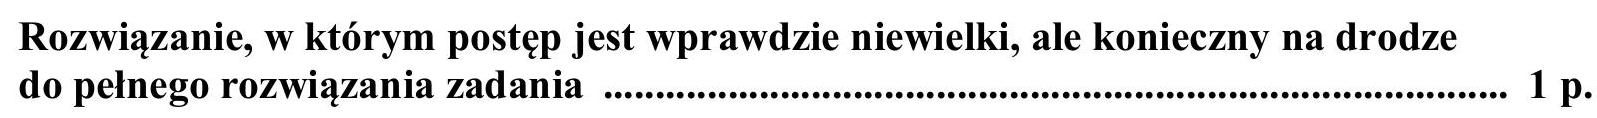
\includegraphics[max width=\textwidth, center]{2025_02_07_cd06b1485e4d114dda29g-28}\\
Zdający uzależni wartości dwie spośród liczb $a, b, c$ od trzeciej z liczb i od różnicy $r$ ciągu arytmetycznego, np.: $a=b-r$ i $c=b+r$ i na tym zakończy lub dalej popełnia błędy.\\
$\qquad$\\
Zdający zapisze równania wynikające z własności ciągu arytmetycznego i z własności ciągu geometrycznego, np.: $a=b-r, c=b+r, b^{2}=(a-2) \cdot(2 c+1)$\\
i na tym zakończy lub dalej popełnia błędy.

Pokonanie zasadniczych trudności zadania 3 p.\\
Zdający zapisze równanie z jedną niewiadomą, wynikające z własności ciągu geometrycznego, np.: $81=(7-r)(2 r+19)$\\
i na tym zakończy lub dalej popełnia błędy.

Rozwiązanie prawie pełne 5 p.\\
Zdający obliczy liczby $a, b, c$ w jednym z możliwych przypadków i na tym zakończy lub dalej popełnia błędy.

\section*{Uwaga}
Jeśli zdający poprawnie rozwiąże równanie kwadratowe, to otrzymuje 4 punkty.

Rozwiązanie pełne ........................................................................................................... 6 p.\\
Zdający obliczy liczby w dwóch przypadkach spełniających warunki zadania: $a=5, b=9$, $c=13$ oraz $a=\frac{31}{2}, b=9, c=\frac{5}{2}$.

\section*{II sposób rozwiązania}
Rozwiązanie, w którym postęp jest wprawdzie niewielki, ale konieczny na drodze do pelnego rozwiązania zadania

$$
\text { Zdający zapisze jedno z równań: } \frac{a+c}{2}=b, b^{2}=(a-2) \cdot(2 c+1) \text {. }
$$

\section*{Rozwiązanie, w którym jest istotny postęp}
 2 p.Zdający zapisze układ trzech równań z trzema niewiadomymi, np.: $\left\{\begin{array}{l}\frac{a+c}{2}=b \\ a+b+c=27 \\ b^{2}=(a-2) \cdot(2 c+1)\end{array}\right.$.\\
Pokonanie zasadniczych trudności zadania 3 p.\\
Zdający zapisze równanie kwadratowe z jedną niewiadomą, $\mathrm{np} .:-2 c^{2}+31 c+16=81$.

\section*{Rozwiązanie prawie pelne 5 p.}
Zdający obliczy liczby $a, b, c$ w jednym z możliwych przypadków i na tym zakończy lub dalej popełnia błędy.

\section*{Uwaga}
Jeśli zdający poprawnie rozwiąże równanie kwadratowe, to otrzymuje 4 punkty.\\
Rozwiązanie pelne\\
6 p.\\
Zdający obliczy liczby w dwóch przypadkach spełniających warunki zadania: $a=5, b=9$, $c=13$ oraz $a=\frac{31}{2}, b=9, c=\frac{5}{2}$.

III sposób rozwiązania\\
Rozwiązanie, w którym postęp jest wprawdzie niewielki, ale konieczny na drodze do calkowitego rozwiązania\\
Zdający zapisze wszystkie wyrazy ciągu arytmetycznego w zależności od jednej z liczb i ilorazu ciągu geometrycznego, np.

$$
a-2, b=(a-2) q, c=\frac{(a-2) q^{2}-1}{2}
$$

i na tym zakończy lub dalej popełni błędy.\\
Rozwiązanie, w którym postęp jest istotny\\
Zdający zapisze układ równań z dwiema niewiadomymi, np.:

$$
a+(a-2) q+\frac{(a-2) q^{2}-1}{2}=27 \text { i }(a-2) q=\frac{2 a+(a-2) q^{2}-1}{4}
$$

i na tym zakończy lub dalej popełni błędy.

Pokonanie zasadniczych trudności zadania\\
Zdający zapisze równanie kwadratowe z jedną niewiadomą, np.:

$$
3\left(2+2 q+q^{2}\right)=51\left(-2+4 q-q^{2}\right)
$$

i na tym zakończy lub dalej popełni błędy.\\
Rozwiązanie prawie pelne\\
Zdający obliczy liczby $a, b$ i $c$ w jednym z możliwych przypadków i na tym zakończy lub dalej popełnia błędy.

\section*{Uwaga}
Jeśli zdający poprawnie rozwiąże równanie kwadratowe, to otrzymuje 4 punkty.

Rozwiązanie pełne .......................................................................................................... 6 p.\\
Zdający zapisze dwa zestawy liczb spełniające warunki zadania: $a=5, b=9$ i $c=13$\\
oraz $a=\frac{31}{2}, b=9$ i $c=\frac{5}{2}$.

\section*{Uwagi (do wszystkich schematów punktowania)}
\begin{enumerate}
  \item Jeżeli zdający myli własności ciągu arytmetycznego z własnościami ciągu geometrycznego, to za całe rozwiązanie otrzymuje 0 punktów.
  \item Jeżeli zdający odgadnie jeden zestaw liczb $a, b, c$, także ze sprawdzeniem warunków zadania, to otrzymuje $\mathbf{0}$ punktów.
\end{enumerate}

Zadanie 15. (0-7)

\begin{center}
\begin{tabular}{|l|l|}
\hline
\begin{tabular}{l}
III. Modelowanie \\
matematyczne. \\
\end{tabular} & \begin{tabular}{l}
11. Rachunek różniczkowy. Zdający stosuje pochodne do \\
rozwiązywania zagadnień optymalizacyjnych (R11.6). \\
\end{tabular} \\
\hline
\end{tabular}
\end{center}

\section*{Przykładowe rozwiązanie}
Niech $r$ oraz $h$ oznaczają, odpowiednio, promień podstawy walca i wysokość walca. Pole $P$ powierzchni całkowitej tego walca jest równe $P=2 \pi r^{2}+2 \pi r h$. Stąd

$$
h=\frac{P-2 \pi r^{2}}{2 \pi r} .
$$

Objętość walca $V=\pi r^{2} h$ zapisujemy jako funkcję zmiennej $r$ :

$$
V(r)=\pi r^{2} \frac{P-2 \pi r^{2}}{2 \pi r}=\frac{P r-2 \pi r^{3}}{2} \text {, gdzie } 0<r<\sqrt{\frac{P}{2 \pi}} .
$$

Pochodna funkcji $V$ jest określona wzorem

$$
V^{\prime}(r)=\frac{1}{2}\left(P-6 \pi r^{2}\right) \text { dla } 0<r<\sqrt{\frac{P}{2 \pi}} .
$$

Wyznaczamy miejsca zerowe i badamy znak pochodnej\\
$V^{\prime}(r)=0$ wtedy i tylko wtedy, gdy $r=\sqrt{\frac{P}{6 \pi}}$,\\
$V^{\prime}(r)>0$ wtedy i tylko wtedy, gdy $0<r<\sqrt{\frac{P}{6 \pi}}$,\\
$V^{\prime}(r)<0$ wtedy i tylko wtedy, gdy $\sqrt{\frac{P}{6 \pi}}<r<\sqrt{\frac{P}{2 \pi}}$.\\
Wynika stąd, że w przedziale $\left(0, \sqrt{\frac{P}{6 \pi}}\right\rangle$ funkcja $V$ jest rosnąca, a w przedziale $\left\langle\sqrt{\frac{P}{6 \pi}}, \sqrt{\frac{P}{2 \pi}}\right)$ jest malejąca. Zatem $V\left(\sqrt{\frac{P}{6 \pi}}\right)$ jest największą wartością tej funkcji. Wartość ta jest równa

$$
V\left(\sqrt{\frac{P}{6 \pi}}\right)=\frac{P \cdot \sqrt{\frac{P}{6 \pi}}-2 \pi \cdot\left(\sqrt{\frac{P}{6 \pi}}\right)^{3}}{2}=\frac{P}{3} \cdot \sqrt{\frac{P}{6 \pi}} .
$$

Gdy $r=\sqrt{\frac{P}{6 \pi}}$, to wtedy $h=\frac{P-2 \pi r^{2}}{2 \pi r}=\sqrt{\frac{2 P}{3 \pi}}$.

\section*{Schemat punktowania}
Rozwiązanie zadania składa się z trzech etapów.\\
a) Pierwszy etap składa się z trzech części:

\begin{itemize}
  \item wyznaczenie wysokością walca w zależności od promienia podstawy walca: $h=\frac{P-2 \pi r^{2}}{2 \pi r}$,
  \item wyznaczenie objętości walca jako funkcji jednej zmiennej $r, V(r)=\frac{P r-2 \pi r^{3}}{2}$,
  \item wyznaczenie dziedziny funkcji $V: D_{V}=\left(0, \sqrt{\frac{P}{2 \pi}}\right)$.
\end{itemize}

Za poprawne wykonanie każdej z tych części zdający otrzymuje 1 punkt.\\
b) Drugi etap składa się z trzech części:

\begin{itemize}
  \item wyznaczenie pochodnej funkcji wielomianowej $f(r)=\frac{P}{2} \cdot r-\pi r^{3}$ :
\end{itemize}

$$
f^{\prime}(r)=\frac{P}{2}-3 \pi r^{2},
$$

\begin{itemize}
  \item obliczenie miejsc zerowych pochodnej funkcji $V: r=\sqrt{\frac{P}{6 \pi}}$ lub obliczenie miejsc zerowych pochodnej funkcjif: $r=-\sqrt{\frac{P}{6 \pi}}, r=\sqrt{\frac{P}{6 \pi}}$.
  \item zbadanie znaku pochodnej funkcji $V$ i uzasadnienie, że dla $r=\sqrt{\frac{P}{6 \pi}}$ funkcja $V$ osiąga największą wartość.
\end{itemize}

Za poprawne rozwiązanie każdej z części tego etapu zdający otrzymuje $\mathbf{1}$ punkt.\\
c) Trzeci etap.

Obliczenie największej objętości walca i wysokości walca o największej objętości:\\
$V=\frac{P}{3} \cdot \sqrt{\frac{P}{6 \pi}}, h=\sqrt{\frac{2 P}{3 \pi}}$.\\
Za poprawne wykonanie tego etapu zdający otrzymuje 1 punkt.

\section*{Uwagi}
\begin{enumerate}
  \item Jeżeli zdający zapisze objętość walca z błędem rzeczowym, to może otrzymać co najwyżej 1 punkt za całe rozwiązanie, a jeżeli dodatkowo poprawnie wyznaczy dziedzinę funkcji $V$, to może otrzymać co najwyżej 2 punkty za całe rozwiązanie.
  \item Jeżeli zdający obliczy pochodną funkcji $f$ lub $V$ z błędem rachunkowym i otrzyma funkcję liniową albo funkcję kwadratową o ujemnym wyróżniku o wyróżniku równym 0 , to może otrzymać punkty jedynie za pierwszy etap rozwiązania.
  \item Jeśli zdający rozwiązuje zadanie dla stożka, to otrzymuje $\mathbf{0}$ punktów, nawet jeśli rozwiązanie tego innego zadania jest poprawne.
  \item Za rozwiązanie z konkretną wartością liczbową w miejsce $P$ zdający otrzymuje 0 punktów.
\end{enumerate}

\end{document}